\chapter{}\label{chap3}

\begin{center}
\rule{5cm}{1pt}\\[5pt]
{\Large\bfseries ಸಮಸ್ಯೆಗಳು}\\[3pt]
\rule{5cm}{1pt}
\end{center}

\smallskip
\begin{enumerate}
\renewcommand{\labelenumi}{\bf\theenumi.}
\itemsep=5pt
\item 1 ರಿಂದ 9ವರೆಗಿನ ಅಂಕಿಗಳನ್ನು ಒಮ್ಮೆ ಮಾತ್ರ ಬಳಸಿ 100 ಬರಿಸಿ. ಯಾವುದೇ ಗಣಿತ ಚಿಹ್ನೆ /ಪ್ರಕ್ರಿಯೆ ಎಷ್ಟು ಬಾರಿ ಬೇಕಾದರೂ ಬಳಸಬಹುದು.

\item ಎಂಟು 8 ಬಳಸಿ 1000 ಬರಿಸಿ ಯಾವುದೇ ಗಣಿತ ಚಿಹ್ನೆ ಬಳಸಬಹುದು.

\item 1, 2, 3, 4, 5, 6, 7 ಗಳನ್ನು ಒಮ್ಮೆ ಮಾತ್ರ ಬಳಸಿ 100 ಬರಿಸಿ ಅಂಕಿಗಳು ಬಿಡಿ ಇಲ್ಲವೇ ಜೋಡಿ ಇರಬಹುದು. ಯಾವುದೇ ಗಣಿತ ಚಿಹ್ನೆ ಬಳಸಬಹುದು.

\item ಐದು ಸಲ 5 ಬಳಸಿ 1  ಬರಿಸಿ. ಯಾವುದೇ ಗಣಿತ ಚಿಹ್ನೆ ಬಳಸಬಹುದು.

\item ಐದು ಸಲ 3 ಬಳಸಿ 31 ಬರಿಸಿ. ಯಾವುದೇ ಗಣಿತ ಚಿಹ್ನೆ  ಬಳಸಬಹುದು. 

\item 2, 3, 4, 5, 6, 7, 8, 9, 10 ಇವುಗಳಿಂದ ಭಾಗಿಸಿದಾಗ, ಭಾಜಕಕ್ಕಿಂತ 1 ಕಡಿಮೆ ಶೇಷ ಕೊಡುವ ಅತಿ ಚಿಕ್ಕ ಸಂಖ್ಯೆ ಯಾವುದು? 

\item ಏಳು ಗೆರೆಗಳಿಂಡ ಸಂಖ್ಯಾ ಸಮೀಕರಣ ರಚಿಸಬಹುದು. 

{\bf ಉದಾ:} II $-$ I = I ಮತ್ತೆರಡು ಉದಾಹರಣೆ ಕೊಡಿ

\item II $-$ IIII = II ಒಂದು ಗೆರೆ ಸ್ಥಾನ ಪಲ್ಲಟ ಮಾಡಿ ಸಮೀಕರಣ ಸರಿದೂಗಿಸಿ. $\neq$ ಬರುವಂತಿಲ್ಲ. (IVಯನ್ನು IIII ಎಂದೂ ಬರೆಯುತ್ತಾರೆ.) 

\item V $-$ IV = VII ಒಂದು ಗೆರೆ ಸ್ಥಾನ ಪಲ್ಲಟ ಮಾಡಿ ಸಮೀಕರಣ ಸರಿದೂಗಿಸಿ. $\neq$ ಬರಬಾರದು.

\item ಹತ್ತೊಂಭತ್ತರಲ್ಲಿ 1 ಕಳೆದರೆ ಇಪ್ಪತ್ತು. ಹೇಗೆ?

\item ಆರು ಬೆಂಕಿಕಡ್ಡಿ ಜೋಡಿಸಿ 100 ಬರಿಸಿ.

\item 6 ಬೆಂಕಿಕಡ್ಡಿ ಜೋಡಿಸಿ ಸಮಷಡ್ಭುಜಾಕೃತಿ ರಚಿಸಿದೆ. ಇನ್ನೂ 3 ಕಡ್ಡಿ  ಸೇರಿಸಿ, 3 ಸಮಾಂತರ ಚತುರ್ಭುಜ ಬರಿಸಿ 

\item 13 ಬೆಂಕಿಕಡ್ಡಿಗಳನ್ನು ಈ ಆಕೃತಿಯಲ್ಲಿ ಜೋಡಿಸಿದೆ. ಯಾವ 4 ಕಡ್ಡಿ ತೆಗೆದರೆ 1 ಟ್ರೆಕೀಜಿ಼ಯಂ, 2 ತ್ರಿಭುಜಗಳು, 1 ಸಮಾಂತರ ಚತುರ್ಭುಜ ಉಳಿಯುತ್ತವೆ?

\begin{figure}[H]
\centering
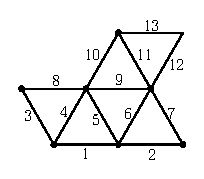
\includegraphics{images/chap3/q13.eps}
\end{figure}

\item 17 ಬೆಂಕಿಕಡ್ಡಿಗಳನ್ನು 6 ಚೌಕಗಳಾಗುವಂತೆ ಜೋಡಿಸಿದೆ. ಅವುಗಳಲ್ಲಿ ಯಾವುದಾದರೂ 5 ಕಡ್ಡಿ ತೆಗೆದು ಹಾಕಿ, ಮೊದಲಿನ  ಗಾತ್ರದ 3 ಚೌಕ ಮಾತ್ರ ಉಳಿಯುವಂತೆ ಮಾಡಿ.

\begin{figure}[H]
\centering
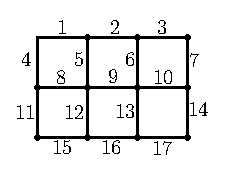
\includegraphics{images/chap3/q14.eps}
\end{figure}

\item 24 ಬೆಂಕಿಕಡ್ಡಿ ಬಳಸಿ 9 ಚೌಕಗಳಾಗುವಂತೆ ಜೋಡಿಸಿದೆ. ಯಾವುದಾದರೂ 4 ಕಡ್ಡಿ ತೆಗೆದು ಹಾಕಿ, ಮೊದಲಿನ ಅಳತೆಯ 5 ಚೌಕಗಳು ಮಾತ್ರ ಉಳಿಯುವಂತೆ ಮಾಡಿ.

\begin{figure}[H]
\centering
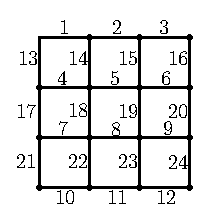
\includegraphics{images/chap3/q15.eps}
\end{figure}

\item 24 ಬೆಂಕಿಕಡ್ಡಿ ಬಳಸಿ 9 ಚೌಕಗಳಾಗುವಂತೆ ಜೋಡಿಸಿದೆ. ಯಾವ 8 ಕಡ್ಡಿ ತೆಗೆದು ಹಾಕಿದರೆ 2 ಚೌಕ ಮಾತ್ರ ಉಳಿಯುತ್ತವೆ? 

\begin{figure}[H]
\centering
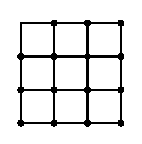
\includegraphics{images/chap3/q16.eps}
\end{figure}

\item ಈ ಗುಣಾಕಾರ ಗಮನಿಸಿ. ಮುಂದಿನ 2 ಹಂತ ಬರೆಯಿರಿ. 
\begin{align*}
3 \times 3 & = 9\\
33 \times 33 & = 1089\\
333 \times 333 & = 110889\\
3333 \times 3333 & = 11108889
\end{align*}

\item ಈ ಗುಣಾಕಾರ ಗಮನಿಸಿ. ಮುಂದಿನ 3 ಹಂತ ಬರೆಯಿರಿ. 
\begin{align*}
1 \times 8 + 1 & = 9\\
12 \times 8 + 2 & = 98\\
123 \times 8 + 3 & = 987\\
1234 \times 8 + 4 & = 9876
\end{align*}

\item ಈ ಗುಣಾಕಾರ ವಿಶಿಷ್ಟತೆ ಗಮನಿಸಿ. 33ರ ಮಗ್ಗಿಯ ಉಳಿದ ಸಂಖ್ಯೆಗಳಿಂದ ಗುಣಿಸಿ, ಉತ್ತರ ತಾಳೆನೋಡಿ 
\begin{align*}
3367 \times 33 & = 111111\\
3367 \times 66 & = 222222\\[0.2cm]
3367 \times 297 & = 999999
\end{align*}

\item ಯಾವ ನಾಲ್ಕು ಅಂಕಿಗಳ ಸಂಖ್ಯೆ ಈ ಸಮೀಕರಣವನ್ನು ಸರಿದೂಗಿಸುತ್ತದೆ? (a, b, c, d ಗಳು ಸೂಚಿಸುವ ಅಂಕಿಗಳು ಯಾವುದು)

4 $\times$ abcd = dcba

\item ಇವುಗಳಲ್ಲಿ ಪ್ರತಿಯೊಂದರಲ್ಲಿಯೂ ಇರುವ ಎಲ್ಲಾ ಅಳತೆಯ ತ್ರಿಭುಜಗಳೆಷ್ಟು?

\begin{figure}[H]
\centering
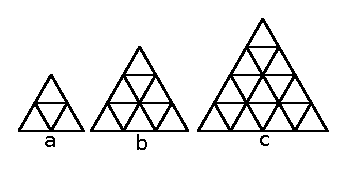
\includegraphics{images/chap3/q21.eps}
\end{figure}

\item ಒಂದು ರಟ್ಟಿನ ಮೇಲೆ 6 ಚೌಕಗಳನ್ನು ಬರೆದು, ಕತ್ತರಿಸಿ. ಇದರಿಂದ 1 ಘನಾಕೃತಿ ರಚಿಸಬಹುದು. ಇದಕ್ಕೆ ಜಾಲ (not) ಎನ್ನುತ್ತಾರೆ. ಒಂದು ಘನಕೃತಿ ರಚಿಸಲು ಎಷ್ಟು ಬೇರೆ ಬೇರೆ ಬಗೆಯ ಜಾಲ ಕತ್ತರಿಸಬಹುದು?

\item ನಾಲ್ಕು ಪಟ್ಟಣಗಳು A, B, C, D 10ಮೈಲಿ ಬಾಹುವಿನ ಚೌಕದ ಮೂಲೆಗಳಲ್ಲಿವೆ. ನಾಲ್ಕನ್ನೂ ಸಂಪರ್ಕಿಸಲು ಹೆದ್ದಾರಿ ನಿರ್ಮಿಸಬೇಕಿದೆ. ಅತಿ ಕಡಿಮೆ ಉದ್ದದ ರಸ್ತೆ ಹೇಗೆ?

\item ಒಬ್ಬ ಬಡಗಿ ಆಟಿಕೆ ತಯಾರಿಸುತ್ತಿದ್ದ. ಒಂದು ಘನಾಕೃತಿ (2') ಮೇಲ್ಮೈಗೆ 1" ಚೌಕದ ಚಿತ್ರಗಳನ್ನು ಅಂಟಿಸಬೇಕಾಗಿತ್ತು. ಆತನಲ್ಲಿದ್ದ ಎಲ್ಲಾ ಚಿತ್ರ ಅಂತಿಸಲು 2" ಘನಾಕೃತಿಯ ಮೇಲ್ಮೈನ 2ರಷ್ಟು ಸ್ಥಳ ಬೇಕೆಂದು ತೋರಿತು. ಅದನ್ನು ಮಾಡಿದ ಹೇಗೆ?

\item ದಾಶಾಂಕು ಶಾಹಿ ಡಮರುಕ ಕಪಾಲ ಶೂಲೈಃ ।

ಬಟ್ವಾಂಗ ಶಕ್ತಿ ಶರ ಚಾತ ಯುತೈರ್ಭವಂತಿ ।।

ಅನ್ಯೋನ್ಯ ಹಸ್ತ ಕಲಿತೈಃ ಕಃ ಮೂರ್ತಿ ಭೇದಾಃ ।

ಶಂಭೋರ್ಹರೇರಿವ ಗದಾರಿ ಸರೋಜ ಖಡ್ಗೈಃ ।।

\hfill (ಭಾಸ್ಕರಾಚಾರ್ಯರ ‘ಲೀಲಾವತಿ’ಯಿಂದ)

{\bf ಅರ್ಥ:} ಪಾಶ, ಅಂಗುಶ, ಸರ್ಪ, ಡಮರುಕ, ಕಪಾಲ, ತ್ರಿಶುಲ, ಡೊಣ್ಣೆ, ಕತ್ತಿ, ಬಾಣ, ಧನಸ್ಸು - ಎಂಬ ಹತ್ತು ಭೂಷಣಗಳನ್ನು ಹತ್ತು ಕೈಗಳಲ್ಲಿ ಬೇರೆ ಬೇರೆ ಕ್ರಮಗಳಲ್ಲಿಟ್ಟು ಶಂಭುವಿನ ಮೂರ್ತಿಗಳನ್ನು ಮಾಡಿದರೆ ಎಷ್ಟು ಮೂರ್ತಿಗಳಾಗುತ್ತವೆ? ಹಾಗೆಯೇ ಗದೆ, ಚಕ್ರ, ಸದ್ಮ, ಕತ್ತಿಗಳ ಹರಿಯ ಮೂರ್ತಿಗಳೆಷ್ಟಾಗುತ್ತವೆ?

\item ಒಂದು ಕಂಭದ $\dfrac{1}{12} \text{ ಭಾಗ}~ \times \dfrac{1}{30}$ ಭಾಗ ನಿರಿನೊಳಗಿದೆ. ಉಳಿದುದರ $\dfrac{1}{20}$ ಭಾಗ ಮತ್ತು ಅದರ $\dfrac{3}{16}$ ಭಾಗ ಕೆಸರಿನಲ್ಲಿ ಹೂತು ಹೋಗಿದೆ. 20 ಮೊಳದಷ್ಟು ಉದ್ದ ಹೊರಗಡೆಲಿದೆ. ಮಿತ್ರನೇ ಕಂಬದ ಉದ್ದವೆಷ್ಟು?

\item ಒಂದು ಜಾನಪದ ಸಮಸ್ಯೆ 

ನೀರೊಳಗೇಳೆಮ್ಮಿ 

ಏರೀಮೇಲ್ಹತ್ತೆಮ್ಮಿ 

ಮನೆಯಾಗ ಹಿಂಡಕೈ ತೊಂದಮ್ಮಿ 

ಒಟ್ಟು ಆದ ಲೇ ಸೆಮ್ಮಿ 

(ಎಮ್ಮೆ - ಎತ್ತು)

\item ಈ ಆಕೃತಿಯಲ್ಲಿ 1 ರಿಂದ 8 ವರೆಗಿನ ಅಂಕಿ ತುಂಬಿಸಬೇಕು. ನೇರವಾಗಿಯಾಗಲೀ, ಅಡ್ಡವಾಗಿಯಾಗಲೀ, ಓರೆಯಾಗಿಯಾಗಲೀ ಅನು ಕ್ರಮ ಸಂಖ್ಯೆ ಬರಬಾರದು. ಹೇಗೆ?

\begin{figure}[H]
\centering
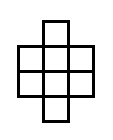
\includegraphics{images/chap3/q28.eps}
\end{figure}

\item ABCDಯು 10cm ಚೌಕ E, F, G, H ಗಳು ಕ್ರಮವಾಗಿ AB, BC, CD, DA ಗಳ ಮಧ್ಯ ಬಿಂದುಗಳು. AF, BG, CH, DE ಸೇರಿಸಿದೆ. 

ಇವುಗಳು ಛೇದಿಸುವ ಬಿಂದುಗಳು P, Q, R, S. 

PQRS ಚೌಕದ ವಿಸ್ತೀರ್ಣ ಲೆಕ್ಕಿಸಿ.

\begin{figure}[H]
\centering
\includegraphics{images/chap3/q29.eps}
\end{figure}

\item ಸಂಖ್ಯಾಹಾರ
\begin{figure}[H]
\centering
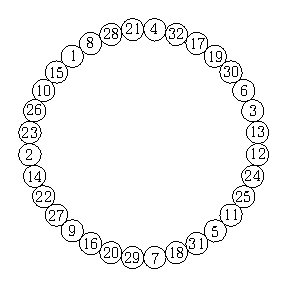
\includegraphics{images/chap3/q30.eps}
\end{figure}

1 ರಿಂದ 32 ವರೆಗಿನ ಸಂಖ್ಯೆಗಳನ್ನು ಒಮ್ಮೆ ಮಾತ್ರ ಬಳಸಿದೆ. ಯಾವುದೇ 2 ಅನುಕ್ರಮ ಸಂಖ್ಯೆ ಕೂಡಿಸಿದರೆ ವರ್ಗಸಂಖ್ಯೆ ಬರುತ್ತದೆ. 

{\bf ಉದಾ:}
\begin{tabular}[t]{rr}
$32 + 17$ & $= 49 = 7^{2}$\\
$14 + 2$ & $= 16 = 4^{2}$\\
$14 + 22$ & $= 36 = 6^{2}$
\end{tabular}

(ಜಪಾನಿ ಗಣಿತಜ್ಞ ನೊಬುಯುಕಿ ಯೋಷಿಗಹಾರ ಅವರ ರಚನೆ NOBUYUKI YOSHI GAHARA)
\end{enumerate}

\smallskip

\begin{center}
\rule{5cm}{1pt}\\[3pt]
{\Large\bfseries ಉತ್ತರಗಳು}\\[-0.1cm]
\rule{5cm}{1pt}
\end{center}

\begin{enumerate}
\item ಇದಕ್ಕೆ ಹಲವು ಉತ್ತರಗಳಿವೆ. ಕೆಳಗೆ 5ನ್ನು ಕೊಟ್ಟಿದೆ.

\begin{tabular}{ll}
$100$ & $= 1 + 2 + 3 + 4 + 5 + 6 + 7 + (8 \times 9)$\\
$100$ & $= 123 - 45 - 67 + 39$\\
$100$ & $= 15 + 36 + 47 + 2 (9 - 8)$\\
$100$ & $= 123 - 4 - 5 - 6 - 7 + 8 - 9$\\ 
$100$ & $= \frac{1}{2} + \frac{6}{4} + \frac{5 + 3}{8} + 97$
\end{tabular}

\smallskip
\item $888 + 88 + 8 + 8 + 8 = 1000$

\item $15 + 36 + 47 + 2 = 100$

\item \{$(5 \div 5) \div (5 \div 5)$\} $\times 5$

\item $3^{3} + 3 + \frac{3}{3} = 27 + 3 + 1 = 31$

\item ಭಾಜಕಕ್ಕಿಂತ 1 ಕಡಿಮೆ ಶೇಷ ಎಂದರೆ 

\begin{tabular}{l}
2 ರಿಂದ ಭಾಗಿಸಿದಾಗ 1 ಶೇಷ\\
3 ರಿಂದ ಭಾಗಿಸಿದಾಗ 2 ಶೇಷ\\
5 ರಿಂದ ಭಾಗಿಸಿದಾಗ 4 ಶೇಷ ಇತ್ಯಾದಿ
\end{tabular}

ಅದು 2, 3, 4, 5, 6, 7, 8, 9, 10 ಇವುಗಳ ಲಸಾಅ ಕ್ಕಿಂತ 1 ಕಡಿಮೆ 

ಲಸಾಅ = 2520

$\therefore$ ಸಂಖ್ಯೆ  2519

\item $1 \times 1 = 1$

$\sqrt{1} = 1$

\item III = IIII $-$ II (= ನ ಒಂದು ಗೆರೆಯನ್ನು - ಮೇಲಿರಿಸಿದೆ)

\item V $-$ IV = $\sqrt{1}$ (VII ಒಂದು ಗೆರೆಯನ್ನು ಅಡ್ಡಲಾಗಿರಿಸಿದೆ)

\item XIX ಇದು 19. ಇದರ ಮಧ್ಯದ 1 ತೆಗೆದು ಹಾಕಿ XX ಇದು ಬಲ  

\item 
\begin{figure}[H]
\centering
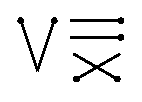
\includegraphics{images/chap3/ans11.eps}
= $\sqrt{10,000} = 100$ \{$\overline{X} = 10000$\}
\end{figure}


\item
%\begin{figure}[H]
%\centering
%\includegraphics{images/chap3/q12.eps}
%\end{figure}

%\begin{figure}[H]
%\centering
%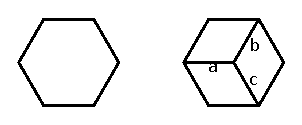
\includegraphics{images/chap3/ans12.eps}
%\end{figure}

\item
\begin{figure}[H]
\centering
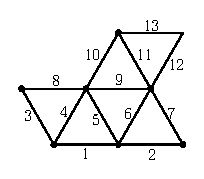
\includegraphics{images/chap3/q13.eps}
\end{figure}

\begin{figure}[H]
\centering
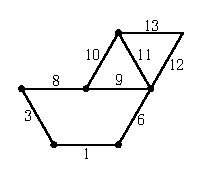
\includegraphics{images/chap3/ans13.eps}
\end{figure}

\item
\begin{figure}[H]
\centering
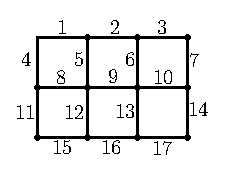
\includegraphics{images/chap3/q14.eps}
\end{figure}

\begin{figure}[H]
\centering
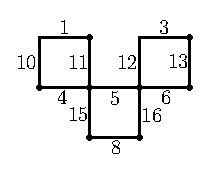
\includegraphics{images/chap3/ans14.eps}
\end{figure}

\item
\begin{figure}[H]
\centering
\includegraphics{images/chap3/ans15a.eps}
\end{figure}


\begin{figure}[H]
\centering
\includegraphics{images/chap3/ans15.eps}
\end{figure}

\item
\begin{figure}[H]
\centering
\includegraphics{images/chap3/ans16a.eps}
\end{figure}

\begin{figure}[H]
\centering
\includegraphics{images/chap3/ans16.eps}
\end{figure}

\item 
\begin{tabular}[t]{rrr}
$3333 \times 3333$ & = & $11108889$\\
$33333 \times 33333$ & = & $1111088889$
\end{tabular}

\smallskip
\item 
\begin{tabular}[t]{rrl}
$12345 \times 8 + 5$ & = & $98765$\\
$123456 \times 8 + 6$ & = & $987654$\\
$1234567 \times 8 + 7$ & = & $9876543$
\end{tabular}

\smallskip
\item
\begin{tabular}[t]{llll}
$3367 \times 99$ & = & $333$ & $333$\\
$3367 \times 132$ & = & $444$ & $444$\\
$3367 \times 165$ & = & $555$ & $555$\\
$3367 \times 198$ & = & $666$ & $666$\\
$3367 \times 231$ & = & $777$ & $777$\\
$3367 \times 264$ & = & $888$ & $888$\\
$3367 \times 297$ & = & $999$ & $999$
\end{tabular}

\item $2178$

\item $a - 5$, $b - 13$, $c - 27$

\item $11$ ಜಾಲಗಳು 
\begin{figure}[H]
\centering
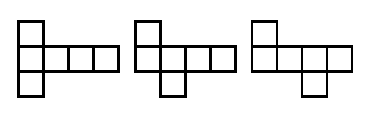
\includegraphics{images/chap3/ans22a.eps}
\includegraphics{images/chap3/ans22b.eps}
\includegraphics{images/chap3/ans22c.eps}
\end{figure}

\item ನಾಲ್ಕು ಪಟ್ಟಣಗಳನ್ನೂ ಸಂಪರ್ಕಿಸುವ ಹಲವು ವಿಧಾನಗಳನ್ನು, ಅವುಗಳ ಉದ್ದವನ್ನೂ ಪರಿಶೀಲಿಸೋಣ
\begin{figure}[H]
\centering
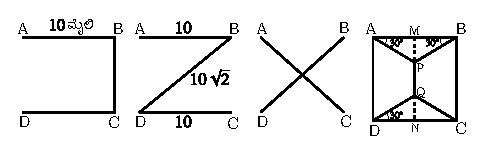
\includegraphics{images/chap3/ans23.eps}
\end{figure}

M, Nಗಳು ABCDಗಳ ಮಧ್ಯ ಬಿಂದುಗಳಾಗಲಿ. 

A ಮತ್ತು D ಗಳಲ್ಲಿ $30^{\circ}$ ಕೋನ ರಚಿಸಿ $\angle{APM} = 60^{\circ}$

$\vartriangle AMP$ಯಲ್ಲಿ $AP = \dfrac{AM}{\sin 60} = \dfrac{5}{0.866} = 5.733$ ಮೈಲಿ 

$\dfrac{AM}{MP} = \tan 60^{\circ}\quad MP = \dfrac{AM}{\tan 60} = \dfrac{5}{\sqrt{6}} = 2.866$ಮೈಲಿ 


$AP = PB = DQ = CQ = 5.733$ ಮೈಲಿ 

$MP + PQ + QN = 10$ ಮೈಲಿ
\begin{align*}
\therefore\quad PQ & = (10 - MP - QN) = (10 - 2.886 - 2.886) ~\text{ ಮೈಲಿ}\\
& = 4.226 ~\text{ ಮೈಲಿ}\\
\therefore\quad \text{ ರಸ್ತೆಯ ಉದ್ದ} & = AB + BP + PQ + QC + QD\\
& = 4 \times 5.773 + 4.266\\
& = 27.38 ~\text{ ಮೈಲಿ}
\end{align*}

ಇದೇ ಅತಿ ಕಡಿಮೆ ದೂರ.

\item 2" ಘನವನ್ನು 1' ಘನಗಳಾಗಿ ಕತ್ತರಿಸಿದ. 8 ಘನಗಳು (1")

2" ಘನದ ಮೇಲ್ಮೈ ವಿಸ್ತೀರ್ಣ = $2^{2} \times 6 = 24$ ಚ. ಅಂ. 

1" ಘನಗಳ ಮೇಲ್ಮೈ ವಿಸ್ತೀರ್ಣ = $8 \times 6 = 48$ ಚ. ಅಂ. 

\item ಇದು ಕ್ರಮ ಸಂಯೋಜನೆಯ ಸಮಸ್ಯೆ (Permutation) 
\begin{align*}
\text{ಶಂಭುವಿನ ವಿಗ್ರಹಗಳು}~ 10~! & = 10 \times 9 \times 8 \times 7 \times 6 \times 5 \times 4 \times 3 \times 2 \times 1\\
& = 36, 28, 800\\
\text{ವಿಷ್ಣುವಿನ ವಿಗ್ರಹಗಳು}~ 4~! & = 4 \times 3 \times 2 \times 1 = 24
\end{align*}

\item ಕಂಬದ ಉದ್ದ $x$ ಇರಲಿ $\left(x - \dfrac{x}{12} \times \dfrac{x}{30}\right) - \dfrac{1}{20} \cdot \dfrac{1}{16} \left(x - \dfrac{x^{2}}{360}\right)^{2} = 20$ ಸಮೀಕರಣ ಲಭಿಸುತ್ತದೆ. 
\begin{align*}
\left(x - \dfrac{x^{2}}{360}\right) - \dfrac{3}{320} \left(x - \dfrac{x^{2}}{360}\right)^{2} & = 20\\
\left(x - \dfrac{x^{2}}{360}\right)^{2} & = p ~\text{ ಇರಲಿ}\\
p - \dfrac{3}{320} p^{2} & = 20
\end{align*}

$320$ ರಿಂದ ಗುಣಿಸಿದಾಗ, $320p - 3p^{2} = 6400$
\begin{gather*}
3p^{2} - 320p + 6400 = 0\\
3p^{2} - 80p - 240p + 6400 = 0\\
p(3p - 80) - 80 (3p - 80) = 0\\
3p - 80 = 0 \ \text{ ಅಥವಾ}\ p - 80 = 0
\end{gather*}

$p = 80$ ಅಥವಾ $p = \frac{80}{3}$

$p = 80$ ತೆಗೆದುಕೊಂಡಾಗ $x - \frac{3x^{2}}{360} = 80$

$360x - 3x^{2} = 28800$ \ ಅಥವಾ \ $3x^{2} - 360x + 28800 = 0$

$(x - 240) (x - 120) = 0$

$\therefore\quad x = 240$ ಅಥವಾ $120$ ಮೊಳಗಳು ಕಂಭದಾತ್ತಾ 

\{$x = \frac{80}{3}$\ ತೆಗೆದುಕೊಂಡರೆ ಅಭಾಗಲಬ್ಧ ಉತ್ತರ ಬರುತ್ತದೆ.\}

\item 1 ಎಮ್ಮೆ ಮಾತ್ರ (ನೀರಿನ ಏಳುತ್ತದೆ, ಏರಿಯ ಮೇಲೆ ಹತ್ತುತ್ತಗೆ, ಮನೆಯಲ್ಲಿ ಹಾಲು ಕೊಡುತ್ತದೆ)

\item 1, 8 ಇದಕ್ಕೆ ಒಂದು ಬದಿಗೆ ಮಾತ್ರ ಅಂಕಿಗಳಿವೆ. ಅವುಗಳನ್ನು ಮಧ್ಯದ ಮನೆಗಳಲ್ಲಿ ಬರೆದು ಉಳಿದ ಅಂಕಿಗಳನ್ನು ಹೊಂದಿಸಿ. 

\begin{figure}[H]
\centering
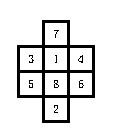
\includegraphics{images/chap3/ans28.eps}
\end{figure}

\item $PQ = x$ ಇರಲಿ  $PQ = QR = RS = SP = x$

$\vartriangle ABQ$ ದಲ್ಲಿ  $E$ ಯು $AB$ ಮಧ್ಯ ಬಿಂದು $PE ||  QB$

$\therefore\quad AP = PQ = x$

ಎಲ್ಲ ಆಕೃತಿಗಳಲ್ಲಿಯೂ $x$ ಗುರ್ತಿಸಿದೆ.  

\begin{figure}[H]
\centering
\includegraphics{images/chap3/ans29.eps}
\end{figure}
\begin{align*}
\vartriangle AQB ~\text{ ದಲ್ಲಿ}\quad AB^{2} & = AQ^{2} + QB^{2}\\
100 & = (AP + PQ)^{2} + QB^{2}\\
& = (2x)^{2} + x^{2}\\
& = 5x^{2}\\
\therefore\quad x^{2} = \frac{100}{5} & = 20 ~\text{ ಚ. ಸೆಂ.ಮೀ}\\
x^{2} & = ABCD - 4 ~\text{ ಟ್ರೆಕೀಜಿ಼ಯಂ} - ೪ ~\text{ ತ್ರಿಭುಜಗಳು}\\
& = ABCD - 4 ~(\text{ ಟ್ರೆಕೀಜಿ಼ಯಂ} + \text{ ತ್ರಿಭುಜ})\\
& \quad\text{ ಟ್ರೆಕೀಜಿ಼ಯಂ} + \text{ ತ್ರಿಭುಜ} = ABCD\\
\therefore x^{2} & = ABCD - 4 ~\text{ ತ್ರಿಭುಜಗಳು} (AQB ~\text{ ಅಳತೆಯವು})\\
\vartriangle AQB & = \frac{1}{2} \cdot 2x = x^{2}\\
\therefore\quad x^{2} & = ABCD - 4x^{2}\\
5x^{2} & = ABCD\\
5x^{2} & = 100\\
x^{2} & = \frac{100}{5} = 20 ~\text{ ಚ. ಸೆಂ.ಮೀ.}
\end{align*}

\item ಉತ್ತರದ ಅಗತ್ಯವಿಲ್ಲ 
\end{enumerate}
